\chapter{Digital signal synthesis}\label{ch:digital_signal_synthesis}

\textit{The previous chapters have covered the physics of our application and
  we were able to recover some technical requirements imposed on our
  implementation. In this chapter we will review the fundamentals of digital
  signal synthesis as \gls{rf} signal source to control the \gls{aod}.
  \gls{dds} offer some distinct advantages over traditional analog
  synthesiser. For one they can cover up a wide frequency range with high
  tuning resolution. In contrast thereto analog devices have to be fitted to
  a narrow operation range and are subject to variations caused by aging,
  thermal drift and manufacturing. In addition \gls{dds} permit extremly fast,
  phase-continous frequency changes, without the loop-settling behaviour
  known to analog devices. Most recently \gls{dds} can easily be integrated
  into existing digital circuits giving rise to a cost-competitive remote
  controllable device. Overall these advantages make the \gls{dds} an
  attractive solution for our projected application \gls{rf} signal source
  \cite{ADTutDDS}.}

\section{Operating principle}

\Cref{fig:dds_simple_architecture} depicts a flow diagram of the components
that make up a simple \gls{dds}. Given a system clock frequency $f_\text{sys}$
and the desired output frequency $f_\text{out}$ one can derive the phase
accumulator increment
\begin{equation}
  \Delta\varphi
  =
  \left\lceil\frac{f_\text{out}}{f_\text{sys}}2^N\right\rceil
  \label{eq:dds_phase_increment}
\end{equation}
where $N$ denotes the number of bits the phase accumulator can store and
$\lceil\cdot\rceil$ is the ceiling function.
\begin{figure}[ht]
  \centering
  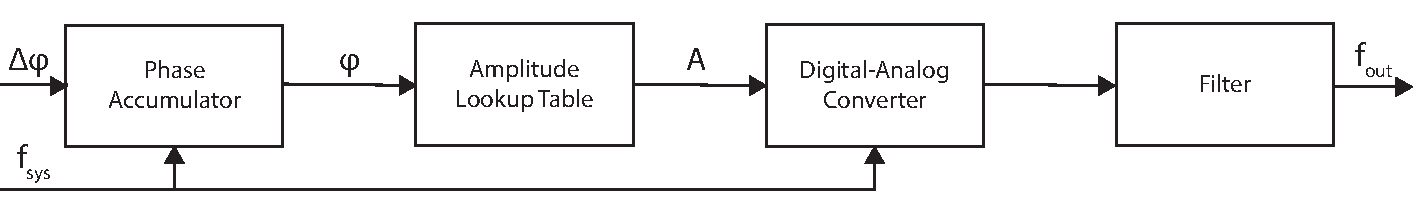
\includegraphics[width=\textwidth]{\figuredir{digital-signal-synthesis/simple-architecture.pdf}}
  \captionsetup{width=.9\textwidth}
  \caption{Signal flow through a simple \gls{dds}. The output frequency
    determines a phase step by which the accumulator is incremented at each
    clock cycle. The value of the phase accumulator is used for amplitude
    lookup of the desired output signal shape. A \gls{dac} outputs the signal
    which then is filtered to smooth the discrete \gls{dac} output.
  }\label{fig:dds_simple_architecture}
\end{figure}
For every clock cycle the phase accumulator is incremented by $\Delta\varphi$.
On overflow of the accumulator a new signal period starts. The phase
accumulator value is used to lookup the corresponding amplitude value of the
desired output signal shape. For example one can use a lookup table with the
values of a sinusoidal output signal. Alternatively one can omit the lookup
table and output a sawtooth output signal by suppling the phase accumulator
output directly to the \gls{dac} or a square wave signal output by suppling
the most significant bit directly. Finally a \gls{dac} converts the digital
amplitude value to an analog signal. An optional analog filter can be used to
smooth the discrete output. In \Cref{fig:dds_simple_output} the signal at the
different processing stages inside a simple \gls{dds} are presented for a
\SI{8}{\bit} precision, system clock frequency
$f_\text{sys}=\SI{1}{\giga\hertz}$ and output frequency
$f_\text{out}=\SI{100}{\mega\hertz}$.
\begin{figure}[ht]
  \centering
  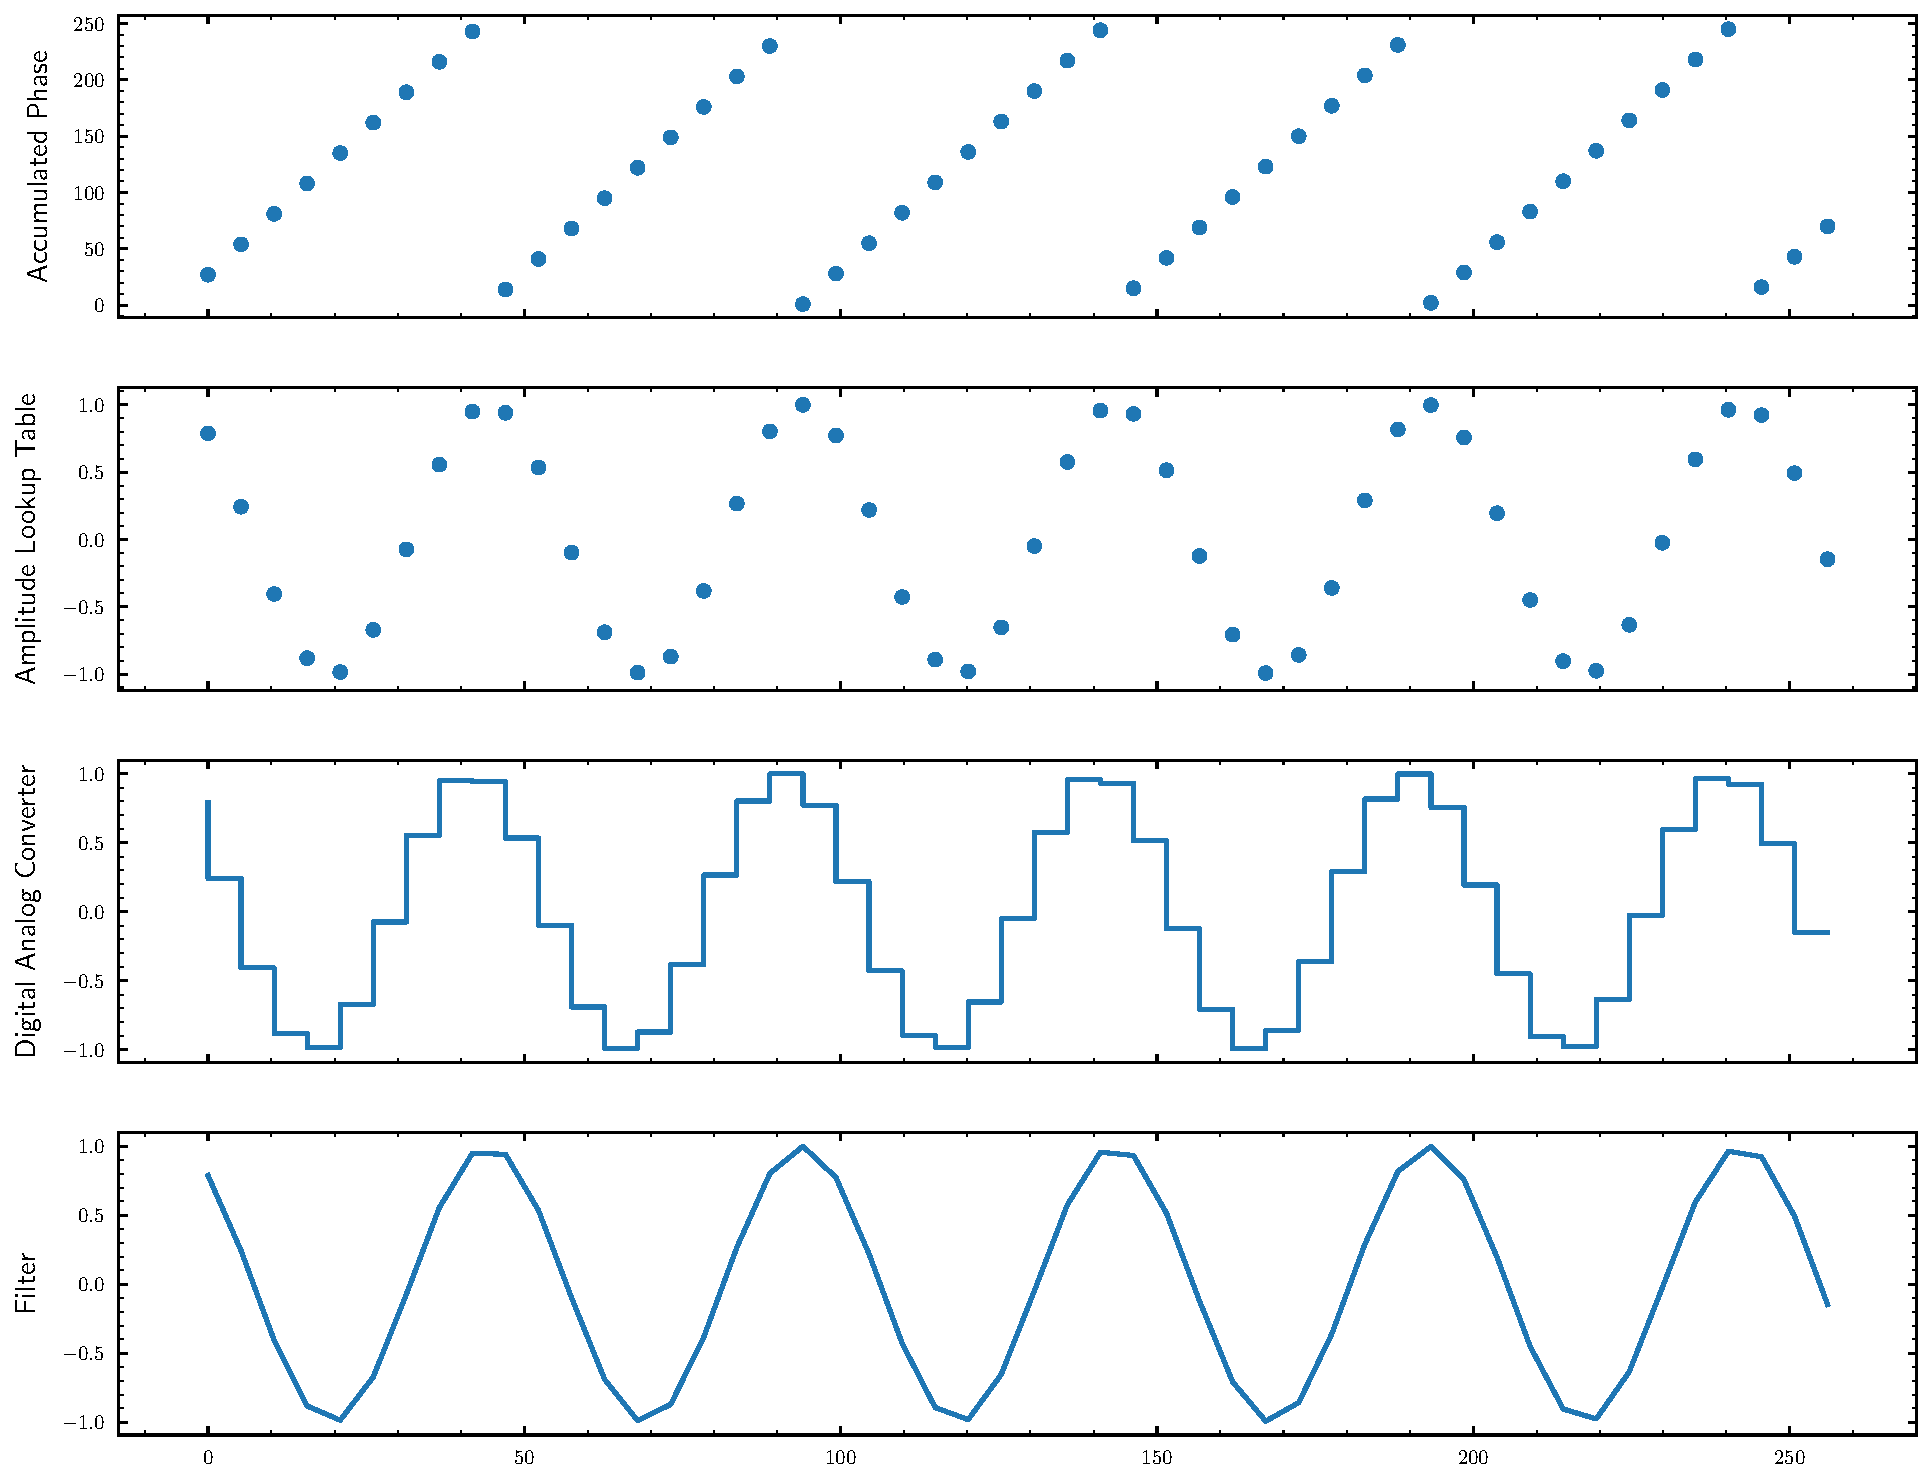
\includegraphics[width=\textwidth]{\figuredir{digital-signal-synthesis/simple-output.pdf}}
  \captionsetup{width=.9\textwidth}
  \caption{Signal outputs at different stages in a simple \gls{dds}. The
    phase accumulator is incremented at each clock cycle by $\Delta\phi$. The
    phase accumulator value is used to lookup a sinusoidal amplitude value
    that is supplied to a \gls{dac}. The final result is smoothed using a
    filter.}\label{fig:dds_simple_output}
\end{figure}
In the first column of \Cref{fig:dds_simple_output} we can see how the phase
accumulator is incremented on every clock iteration and resets on overflow.
In the second column the lookup table has been used to return the
corresponding cosine amplitude. We can see a difference in output shape
between even and odd samples. This is caused by the fact that the phase
increment is not a divisor of the phase accumulator size and we will later
discuss workarounds.

\subsection{Clock generation}

The Nyquist-Shannon sampling theorem states that for a given sample rate a
perfect reconstruction is guaranteed possible for
$f_\text{out}<f_\text{samp}/2$. Until now we have considered the system clock
frequency $f_\text{sys}=f_\text{samp}$ as given. In practice reliable
reference signals are clocked below the desired output range and thereby
cannot directly be used as system clock according to the Nyquist-Shannon
sampling theorem.
\begin{figure}[ht]
  \centering
  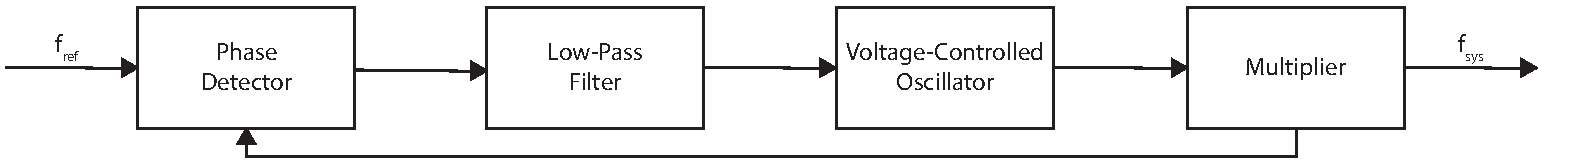
\includegraphics[width=\textwidth]{\figuredir{digital-signal-synthesis/clock-generation.pdf}}
  \captionsetup{width=.9\textwidth}
  \caption{Clock generation signal generation with \gls{pll} and multiplier.
    The phase detector compares the output system phase with the reference
    phase and yields a non-linear error response. The low-pass filter removes
    fast oscillations. The \gls{vco} changes the output phase in dependence
    of the error response. Finally system and reference phase will go in lock.
    }\label{fig:dds_clock_generation}
\end{figure}
\Cref{fig:dds_clock_generation} the system clock generation from a reference
signal is illustrated. The phase detector yields a non-linear error response
comparing the output signal phase with the reference signal phase. After a
low-pass filter removes fast oscillations a \gls{vco} changes its phase
proportional to the error signal. Finally a frequency multiplier creates
harmonics of the reference frequency and extracts a programmed frequency
multiple of $M$ such that the system frequency relates to the reference
clock by $f_\text{sys}=Mf_\text{ref}$ with $1<M\in\mathbb{N}$.

\subsection{Parameter modulation}

So far we only discussed the case of frequency modulation. We will see that
the previous architecture can be easily extended to support amplitude
and phase modulation too.
\begin{figure}[ht]
  \centering
  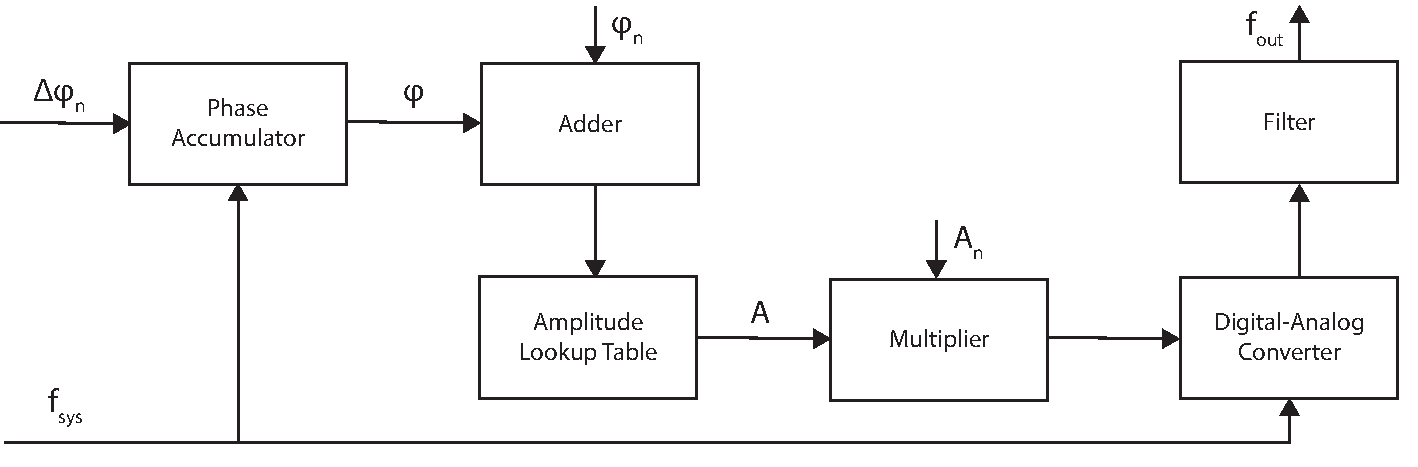
\includegraphics[width=\textwidth]{\figuredir{digital-signal-synthesis/modulation-architecture.pdf}}
  \captionsetup{width=.9\textwidth}
  \caption{\gls{dds} architecture supporting modulation of frequency,
    amplitude and phase offset parameters. Phase accumulator increment is now
    time dependent. The phase offset is also time dependent is added as last
    step to the phase accumulator before supplied to the \gls{dac}. The time
    dependent amplitude parameter is multiplied with the amplitude obtained
    from the lookup table.
    }\label{fig:dds_modulation_architecture}
\end{figure}
In \Cref{fig:dds_modulation_architecture} we can see one realization of an
architecture that supports amplitude, frequency and phase modulation. The main
components are the same as in \Cref{fig:dds_simple_architecture}. In addition
we have an adder for a time dependent phase offset and a multiplier for the
digital amplitude value obtained from the lookup table. The time dependence
of the parameters can be either determined by reading from memory or through
generation of another circuit. In a later section we will discuss the case of
a linear frequency sweep provided by a digital ramp.

\section{Quantization effects}

At the beginning of this chapter we elaborated greatly on the advantages that
digital signal synthesis has to offer. Yet we know that every technical design
involves its unqiue set of compromises. One important part in any engineering
process is to carefully evaluate the implications of these compromises. In
that sense we will discuss the side-effects arising from the digital nature of
digital signal synthesis and what methods there exists to reduce them.

\subsubsection{Phase jitter}

Phase jitter is created when one configures an output frequency for which
$\Delta\varphi$ is not a divider of $2^N$. In this case a phase error of
$-\varphi/(\Delta\varphi)$ builds up until it reaches a full clock period. One
method to circumvent the phase error is to add a delay line after the phase
accumulator\cite{Vankka2013}.

\subsubsection{Phase truncation}

Phase truncation occurs because the amplitude lookup table usually has a
reduced precision $P$ compared to the phase accumulator. The reduced precision
is necessary as most phase accumulators in \gls{dds} nowadays have at least 
$N=\SI{32}{\bit}$ entries and a lookup table supporting that many entries at
high frequencies becomes impractical\cite{Cordesses2004}. Fortunately there
are many procedures to use the limited memory of a sinewave lookup table
more efficiently. For example one can reduce the sinewave data to the domain
from $0$ to $\pi/4$ and use symmetry to infer the values from $\pi/4$ to
$2\pi$. Sophisticated compressions methods allow compression ratios up to
165:1\cite{Cordesses2004} so that in practice phase truncation is not a
problem.

There of course exists many more sources of signal imperfection from which
many can be described analytically \cite{Goldberg1994}. 

\section{Frequency response}

In the previous section we discussed how the signal amplitude deviates from
the ideal amplitude because of reduced precision. In addition the theory of
digital signal synthesis describes a sinc dependency of the amplitude with
respect to frequency caused by the finite precision of the \gls{dac}. The
sinc response can be easily modulated by the zero-order hold model used
in signal processing. The zero-order hold model assumes that a signal $x(t)$
is reconstructed by a piecewise linear approximation
\begin{equation}
  x(t)
  \approx
  \sum_{n\in\mathbb{Z}}x_n\theta\left(\frac{t}{T}-\frac{1-2n}{2}\right)

\end{equation}
where $\theta(t)$ denotes the Heaviside function.

\section{Frequency resolution}

We apply a reference signal of
\begin{equation}
  f_\text{ref}=\SI{10}{\mega\hertz}
\end{equation}
configured to be used with a \gls{pll} multiplier of
$N=100$ yielding a system clock of
\begin{equation}
  f_\text{sys}=Nf_\text{ref}=\SI{1}{\giga\hertz}.
\end{equation}
The timer clock used for the linear ramp and memory playback runs with
a quarter of the system clock
\begin{equation}
  f_\text{timer}=f_\text{sys}/4=\SI{250}{\mega\hertz}.
\end{equation}

The \gls{ad9910} uses a \SI{14}{\bit} \gls{asf} and \SI{32}{\bit} \gls{ftw}
to parameterize amplitude $A(t)$ and output frequency $f(t)$ by
\begin{align}
  FTW
  :=
  \left\lfloor2^{32}\left(\frac{f_\text{out}}{f_\text{sys}}\right)\right\rceil
  &&
  ASF
  :=
  \left\lfloor\frac{A_\text{out}}{2^{14}}\right\rceil
  \label{eq:elec:ftwasf}
\end{align}
wherein $\lfloor{\cdot}\rceil$ rounds the given float to the nearest integer.
The theoretical limit for the maximum output frequency then is found via
\begin{equation*}
  f_\text{max}
  =
  \left(1-\frac{2^{31}-1}{2^{32}}\right)f_\text{sys}
  =
  \left(\frac{1}{2}-\frac{1}{2^{31}}\right)f_\text{sys}
  \approx
  \frac{1}{2}f_\text{sys}
  =
  \SI{500}{\mega\hertz}.
\end{equation*}
Yet the datasheet \cite{AD9910} reports $f_\text{max}=\SI{420}{\mega\hertz}$
and in fact we found the output signal to be very noisy at the theoretical
limit.

We continue with the assessment of the digital ramp that does a unidrectional
linear sweep on the frequency from \SI{90}{\mega\hertz} to
\SI{110}{\mega\hertz}. The digital ramp of the \gls{ad9910} lets us define
a \gls{ftw} step $M$ word of \SI{32}{\bit} as well as a step rate word $S$ of
\SI{16}{\bit} resolution. They relate to the frequency step and the time
step through
\begin{align}
  \Delta f
  =
  \frac{M}{2^{32}}f_\text{sys}
  &&
  \Delta t
  =
  \frac{S}{f_\text{timer}}
  =
  \frac{S}{4f_\text{sys}}.
  \label{eq:elec:step}
\end{align}
The sweep duration is deterimened by $S,M$ through
\begin{equation}
  T_\text{duration}
  =
  \frac{f_\text{upper}-f_\text{lower}}{\Delta f}\Delta t
  =
  2^{32}\frac{f_\text{upper}-f_\text{lower}}{f_\text{sys}}\frac{S/M}{f_\text{timer}}
\end{equation}
for a target sweep duration of $T_\text{duration}=\SI{10}{ms}$ we find
\begin{equation*}
  \frac{S}{M}
  =
  \frac{T f_\text{timer}}{2^{32}}\frac{f_\text{sys}}{f_\text{upper}-f_\text{lower}}
  =
  \frac{10^9}{2^{35}}
  \approx
  \num{2.9104e-2}
  =
  \frac{1819}{62500}
\end{equation*}
the last step can be obtained by best ratio approximation using continued
fractions as for example described in \cite{Ashley2003}. It should be kept in
mind that the best ratio approximation is likable to introduce an error,
therefore realistic durations may differ from the configured value and it
is possible that better approximations exist that allow smaller $\Delta f,
\Delta t$, thus providing a sweep resolution. In the above case the given
time duration translates to
\begin{align*}
  \Delta f
  =
  \frac{62500}{2^{32}}f_\text{sys}
  \approx
  \SI{145}{\kilo\hertz}
  &&
  \Delta t
  =
  \frac{1819}{f_\text{timer}}
  \approx
  \SI{7.28}{\micro\second}
\end{align*}
or $(f_\text{upper}-f_\text{lower})/\Delta f=138$ discrete data points.

Eventually we are left with the assessment of the amplitude sequence. The
memory fits at most 1024 discrete amplitude values and the \gls{ad9910}
allows us to set the time spent at each amplitude value via the \SI{16}{\bit}
playback rate $P$ word
\begin{equation}
  \Delta t
  =
  \frac{P}{f_\text{timer}}
  =
  \frac{4P}{f_\text{sys}}
\end{equation}
which gives us range from $\min\Delta t=\SI{4}{\nano\second}$ to
$\max\Delta t=\SI{26.14}{\micro\second}$. As we incorporate all of the 1024
data points this gives us a duration range from about
$\min T=\SI{4}{\micro\second}$ to $\max T=\SI{26.84}{\milli\second}$.

